\section{TỔNG VÀ HIỆU CỦA HAI VECTƠ}

\subsection{TÓM TẮT LÝ THUYẾT}
\subsubsection{Vectơ bằng nhau, vectơ đối nhau}
\begin{tcolorbox}[colframe=orange,colback=white,boxrule=0.2mm]
	\begin{itemize}
		\item  Hai vec tơ bằng nhau nếu chúng có cùng \textbf{độ lớn} và \textbf{cùng hướng}.
		\item  Hai vec tơ đối nhau nếu chúng có cùng \textbf{độ lớn} nhưng \textbf{ngược hướng}.
	\end{itemize}
\end{tcolorbox}
\vspace{-0.4cm}
	\immini{\indamm{Ví dụ:} Cho hình bình hành $ABCD$ tâm $O$, ta có vài kết quả sau
	\begin{itemize}
		\item [$\bullet$] Các vectơ bằng nhau $\overrightarrow{AB}=\overrightarrow{DC};\text{}\overrightarrow{AD}=\overrightarrow{BC};$ 
		$\overrightarrow{AO}=\overrightarrow{OC}$; $\overrightarrow{DO}=\overrightarrow{OB}$,...
		\item [$\bullet$] Các vectơ đối nhau: $\overrightarrow{AB}$ đối $\overrightarrow{CD}$; $\overrightarrow{BC}$ đối $\overrightarrow{DA}$; $\overrightarrow{OA}$ đối $\overrightarrow{OC}$; $\overrightarrow{OB}$ đối $\overrightarrow{OD}$;...
	\end{itemize}
}{\hspace{1cm}
\begin{tikzpicture}[scale=1, line join=round, line cap=round]
	\tkzDefPoints{0/0/A,4/0/B,5/2/C}
	\tkzDefPointBy[translation=from B to C](A)\tkzGetPoint{D}
	\tkzInterLL(A,C)(B,D)\tkzGetPoint{O}
	\tkzDrawSegments(A,B B,C C,D D,A A,C B,D)
	\tkzDrawPoints[size=2,fill=black](A,B,C,D,O)
	\tkzLabelPoints[below,font=\footnotesize](A, B, O)
	\tkzLabelPoints[above,font=\footnotesize](C,D)
	\node[below] at (2,-0.5) {Hình 1};
\end{tikzpicture}}
\subsubsection{Phép toán cộng hai vectơ}
Phép cộng hai vectơ có tính chất giao hoán. Khi thực hiện phép toán cộng hai vec tơ, ta chú ý các quy tắc sau

\begin{itemize}
	\item [\iconMT] \indam{Quy tắc 3 điểm:}
	\begin{boxkn}
	\immini{Với ba điểm $A,B,C$ bất kì, ta luôn có
		\fbox{$\overrightarrow{AB}+\overrightarrow{BC}=\overrightarrow{AC}$}
		\begin{itemize}
			\item [$\bullet$] Dấu hiệu nhận biết là "điểm liên tiếp nhau".
			\item [$\bullet$] Các hệ thức tương tự
			\begin{listEX}[2]
				\item [] $\overrightarrow{BA}+\overrightarrow{AC}=\overrightarrow{BC}$
				\item [] $\overrightarrow{CB}+\overrightarrow{BA}=\overrightarrow{CA}$
			\end{listEX}
		\end{itemize}
		
	}{\hspace{1cm}
	\begin{tikzpicture}[scale=0.6, line join=round, line cap=round]
	\tkzDefPoints{0/0/A,5/0/C,2/2/B}
	\tkzDrawSegments(A,B B,C C,A)
	\tkzDrawPoints[size=2,fill=black](A,B,C)
	\tkzLabelPoints[above](B)
	\tkzLabelPoints[below](A,C)
	\end{tikzpicture}}
\end{boxkn}
	\item [\iconMT] \indam{Quy tắc hình bình hành:}
	\begin{boxkn}
	\immini{Xét hình bình hành $ABCD$, ta luôn có
		\fbox{$\overrightarrow{AB}+\overrightarrow{AD}=\overrightarrow{AC}$}
		\begin{itemize}
			\item [$\bullet$] Dấu hiệu nhận biết là "cùng gốc".
			\item [$\bullet$] Các hệ thức tương tự
			\begin{listEX}[2]
				\item [] $\overrightarrow{BA}+\overrightarrow{BC}=\overrightarrow{BD}$
				\item [] $\overrightarrow{CB}+\overrightarrow{CD}=\overrightarrow{CA}$
			\end{listEX}
		\end{itemize}
		
	}{\hspace{1cm}
		\begin{tikzpicture}[scale=0.6, line join=round, line cap=round]
		\tkzDefPoints{0/0/A,1/2/B,5/2/C,4/0/D}
		\tkzDrawSegments(A,B B,C C,D D,A)
		\tkzDrawPoints[size=2,fill=black](A,B,C,D)
		\tkzLabelPoints[below](A,D)
		\tkzLabelPoints[above](B,C)
		\end{tikzpicture}}
	\end{boxkn}
	\item [\iconMT] \indam{Quy tắc cộng vectơ đối:}
	\begin{boxkn}
	\begin{itemize}
		\item [$\bullet$] Nếu $\overrightarrow{a}$ và $\overrightarrow{b}$ đối nhau thì $\overrightarrow{a}+\overrightarrow{b}=\overrightarrow{0}$.
		\item [$\bullet$] Trong Hình 1 ở trên, ta có
		\begin{listEX}[3]
			\item [] $\overrightarrow{AD}+\overrightarrow{CB}=\overrightarrow{0}$
			\item [] $\overrightarrow{AB}+\overrightarrow{CD}=\overrightarrow{0}$
			\item [] $\overrightarrow{OA}+\overrightarrow{OC}=\overrightarrow{0}$
		\end{listEX}
	\end{itemize} 
\end{boxkn}
\indamm{Tính chất:} Với ba vectơ $\vec{a}$, $\vec{b}$, $\vec{c}$ tùy ý
\begin{tcolorbox}[colframe=orange,colback=white,boxrule=0.2mm]
	\begin{itemize}
		\item Tính chất giáo hoán: $\vec{a}+\vec{b}=\vec{b}+\vec{a}$.
		\item Tính chất kết hợp: $(\vec{a}+\vec{b})+\vec{c}=\vec{a}+(\vec{b}+\vec{c})$.
		\item Tính chất của vectơ-không: $\vec{a}+\vec{0}=\vec{a}$.
	\end{itemize}
\end{tcolorbox}
\end{itemize}
\subsubsection{Phép toán hiệu hai vectơ}
	\begin{itemize}
		\item [\iconMT] \indam{Vectơ đối:} 
		\begin{itemize}
			\item [$\bullet$] Vectơ đối của $\vec{a}$ kí hiệu là $-\vec{a}$.
			\item [$\bullet$] Vectơ đối của $\overrightarrow{AB}$ là $\overrightarrow{BA}$, nghĩa là \fbox{$-\overrightarrow{AB}=\overrightarrow{BA}$} (\textit{dùng để làm mất dấu trừ trước vectơ}).
			\item [$\bullet$] Vectơ $\vec{0}$ được coi là vectơ đối của chính nó.
		\end{itemize} 
		\item [\iconMT] \indam{ Quy tắc trừ:} Với ba điểm $A,B,C$ bất kì, ta luôn có
		\fbox{$\overrightarrow{BC}=\overrightarrow{AC}-\overrightarrow{AB}$}
	\end{itemize}
\subsubsection{Công thức trung điểm, trọng tâm}
\begin{itemize}
	\item [\iconMT] \indam{Công thức trung điểm:}
\immini{\begin{itemize}
		\item [$\bullet$] Nếu $M$ là trung điểm của đoạn $AB$ thì $\overrightarrow{MA}+\overrightarrow{MB}=\overrightarrow{0}$.
		\item [$\bullet$] Tương tự $\overrightarrow{AM}+\overrightarrow{BM}=\overrightarrow{0}$.
	\end{itemize} }{
	\begin{tikzpicture}[scale=1, line join=round, line cap=round]
		\tikzset{label style/.style={font=\footnotesize}}
		\tkzDefPoints{0/0/A,4/0/B}
		\coordinate (M) at ($(A)!0.5!(B)$);
		\tkzDrawPoints[size=2,fill=black](A,B,M)
		\tkzDrawSegments(A,B)
		\tkzLabelPoints[above](A,B,M)	
\end{tikzpicture}}
	\item [\iconMT] \indam{Công thức trọng tâm:}
\immini{\begin{itemize}
		\item [$\bullet$] Nếu $G$ là trọng tâm của tam giác $ABC$ thì $$\overrightarrow{GA}+\overrightarrow{GB}+\overrightarrow{GC}=\overrightarrow{0}.$$
		\item [$\bullet$] Tương tự $\overrightarrow{AG}+\overrightarrow{BG}+\overrightarrow{CG}=\overrightarrow{0}$.
	\end{itemize} }{
		\begin{tikzpicture}[scale=1, line join=round, line cap=round]
		\tikzset{label style/.style={font=\footnotesize}}
		\tkzDefPoints{0/0/B,4/0/C,1/2/A}
		\coordinate (I) at ($(C)!0.5!(B)$);
		\coordinate (K) at ($(A)!0.5!(B)$);
		\coordinate (M) at ($(C)!0.5!(A)$);
		\tkzInterLL(A,I)(C,K)\tkzGetPoint{G}
		\tkzDrawSegments(A,B B,C C,A A,I C,K B,M)
		\tkzDrawPoints[size=2,fill=black](A,B,C,I,K,M,G)
		\tkzLabelPoints[below](C, B,I)
		\tkzLabelPoints[above](A)
		\tkzLabelPoints[above right](M)
		\tkzLabelPoints[above left](K)
		\tkzLabelPoints[above right](G)
\end{tikzpicture}}
\end{itemize}
\subsection{RÈN LUYỆN KĨ NĂNG GIẢI TOÁN}
\begin{dang}{Thực hiện phép toán cộng, trừ hai vectơ}
	\begin{itemize}
		\item [\iconMT] Nếu hai véc tơ được sắp xếp thỏa mãn một trong các quy tắc (ba điểm, hình bình hành, vec tơ đối), thì ta tiến hành phép cộng theo quy tắc tương ứng.
		\item [\iconMT] Nếu hai véc tơ được sắp xếp chưa thỏa mãn quy tắc (điểm chưa liên tiếp, chưa cùng gốc), thì ta tiến hành dời;
		\begin{itemize}
			\item Đề không cho hình vẽ (điểm bất kì), ta dùng quy tắc 3 điểm để chèn điểm vào.
			\item Đề cho hình vẽ (tam giác, hình bình hành,...), ta dùng vectơ bằng nhau, thay vec tơ này bởi vec tơ khác bằng với nó sao cho có thể ghép được "quy tắc cộng" với các véc tơ còn lại.
		\end{itemize}
	\end{itemize}
\end{dang}
\begin{vd}
	\immini{Cho tam giác $ABC$. Các điểm $M$, $N$ và $K$ lần lượt là trung điểm của $AB$, $AC$ và $BC$.
	\begin{tasks}(1)
		\task Tìm các vectơ bằng với $\overrightarrow{MK}$.
		\task Tìm các vectơ đối của $\overrightarrow{MN}$.
		\task  Xác định các véc tơ $\overrightarrow{AM}+\overrightarrow{MN}$;\quad $\overrightarrow{AM}+\overrightarrow{NK}$;\quad $\overrightarrow{AM}+\overrightarrow{KN}$;\quad $\overrightarrow{AM}-\overrightarrow{AN}$; \quad $\overrightarrow{MN}-\overrightarrow{NC}$;\quad $\overrightarrow{BK}-\overrightarrow{CK}$.
	\end{tasks}}{\hspace{1cm}
		\begin{tikzpicture}[scale=1, line join=round, line cap=round]
	\tkzDefPoints{0/0/A,1/2/B,4/0/C}
	\coordinate (M) at ($(A)!0.5!(B)$);
	\coordinate (N) at ($(C)!0.5!(A)$);
	\coordinate (K) at ($(B)!0.5!(C)$);
	\tkzDrawSegments(A,B B,C C,A)
	\tkzDrawPoints[size=2,fill=black](A,B,C,M,N,K)
	\tkzLabelPoints[below, font=\footnotesize](A,N,C)
	\tkzLabelPoints[above, font=\footnotesize](B)
	\tkzLabelPoints[above left, font=\footnotesize](M)
	\tkzLabelPoints[above right, font=\footnotesize](K)
	\end{tikzpicture}}
		\loigiai{
		Vì $M, N, K$ lần lượt là trung điểm của $AB, AC, BC$ nên $MN, NK, MK$ là các đường trung bình của tam giác $ABC$.
		\begin{itemize}
			\item $MK \parallel AC$ và $MK = \dfrac{1}{2}AC = AN = NC$.
			\item $MN \parallel BC$ và $MN = \dfrac{1}{2}BC = BK = KC$.
			\item $NK \parallel AB$ và $NK = \dfrac{1}{2}AB = AM = MB$.
		\end{itemize}
		\begin{enumerate}
			\item[a)] Các vectơ bằng với $\overrightarrow{MK}$ là: $\overrightarrow{AN}$ và $\overrightarrow{NC}$.
			\item[b)] Các vectơ đối của $\overrightarrow{MN}$ là: $\overrightarrow{NM}$, $\overrightarrow{KB}$ và $\overrightarrow{CK}$.
			\item[c)] Ta thực hiện các phép toán vectơ:
			\begin{itemize}
				\item $\overrightarrow{AM} + \overrightarrow{MN} = \overrightarrow{AN}$ (quy tắc ba điểm).
				\item Vì $\overrightarrow{NK} = \overrightarrow{MB}$ nên $\overrightarrow{AM} + \overrightarrow{NK} = \overrightarrow{AM} + \overrightarrow{MB} = \overrightarrow{AB}$.
				\item Vì $\overrightarrow{KN} = \overrightarrow{MA}$ nên $\overrightarrow{AM} + \overrightarrow{KN} = \overrightarrow{AM} + \overrightarrow{MA} = \overrightarrow{AA} = \vec{0}$.
				\item $\overrightarrow{AM} - \overrightarrow{AN} = \overrightarrow{NM}$ (quy tắc trừ).
				\item Vì $N$ là trung điểm $AC$ nên $\overrightarrow{NC} = \overrightarrow{AN}$. Do đó: $\overrightarrow{MN} - \overrightarrow{NC} = \overrightarrow{MN} - \overrightarrow{AN} = \overrightarrow{MN} + \overrightarrow{NA} = \overrightarrow{MA}$.
				\item $\overrightarrow{BK} - \overrightarrow{CK} = \overrightarrow{BK} + \overrightarrow{KC} = \overrightarrow{BC}$.
			\end{itemize}
		\end{enumerate}
	}
\end{vd} \dongcham{8}

\begin{vd}
	\immini{Cho hình bình hành $ABCD$ tâm $O$. 
		\begin{tasks}(1)
			\task Tìm  vectơ bằng với $\overrightarrow{OC}$.
			\task Xác định các vectơ $\overrightarrow{OA}+\overrightarrow{OC}$;\quad $\overrightarrow{OB}+\overrightarrow{OD}$;\quad $\overrightarrow{AB}+\overrightarrow{CD}$;\quad $\overrightarrow{AD}-\overrightarrow{BC}$;\quad $\overrightarrow{OA}+\overrightarrow{DC}$ .
		\end{tasks}
}{\hspace{1cm}
		\begin{tikzpicture}[scale=1, line join=round, line cap=round]
	\tkzDefPoints{0/0/A,1/2/B,5/2/C,4/0/D}
	\tkzInterLL(A,C)(B,D)\tkzGetPoint{O}
	\tkzDrawSegments(A,B B,C C,D D,A A,C B,D)
	\tkzDrawPoints[size=2,fill=black](A,B,C,D,O)
	\tkzLabelPoints[below, font=\footnotesize](A,D)
	\tkzLabelPoints[above, font=\footnotesize](B,C,O)
	\end{tikzpicture}}
	\loigiai{
	Vì $ABCD$ là hình bình hành tâm $O$ nên $O$ là trung điểm của $AC$ và $BD$. Đồng thời các cặp cạnh đối song song và bằng nhau.
	\begin{enumerate}
		\item[a)] Vectơ bằng với $\overrightarrow{OC}$ là $\overrightarrow{AO}$.
		\item[b)] Ta thực hiện các phép toán:
		\begin{itemize}
			\item $\overrightarrow{OA} + \overrightarrow{OC} = \vec{0}$ (do $O$ là trung điểm $AC$, $\overrightarrow{OA}$ và $\overrightarrow{OC}$ là hai vectơ đối nhau).
			\item $\overrightarrow{OB} + \overrightarrow{OD} = \vec{0}$ (do $O$ là trung điểm $BD$).
			\item $\overrightarrow{AB} + \overrightarrow{CD} = \overrightarrow{AB} - \overrightarrow{DC} = \overrightarrow{AB} - \overrightarrow{AB} = \vec{0}$ (vì $\overrightarrow{CD} = -\overrightarrow{DC} = -\overrightarrow{AB}$).
			\item $\overrightarrow{AD} - \overrightarrow{BC} = \overrightarrow{AD} - \overrightarrow{AD} = \vec{0}$ (vì $\overrightarrow{BC} = \overrightarrow{AD}$).
			\item Vì $\overrightarrow{DC} = \overrightarrow{AB}$ nên $\overrightarrow{OA} + \overrightarrow{DC} = \overrightarrow{OA} + \overrightarrow{AB} = \overrightarrow{OB}$.
		\end{itemize}
	\end{enumerate}
}
\end{vd} \dongcham{7}


\begin{vd}
\immini{Cho hình bình hành $ABCD$ Hai điểm $M$ và $N$ lần lượt là trung điểm của $BC$ và $AD$ Xác định vectơ
	\begin{listEX}[2]
		\item [] $\overrightarrow{DA}+\overrightarrow{DC}$,
		\item [] $\overrightarrow{AM}+\overrightarrow{AN}$,
		\item [] $\overrightarrow{AN}+\overrightarrow{CM}$,
		\item [] $\overrightarrow{MB}+\overrightarrow{NC}$.
	\end{listEX}    
}{\hspace{1cm}
		\begin{tikzpicture}[scale=0.9, line join=round, line cap=round]
	\tkzDefPoints{0/0/A,1/2/B,5/2/C,4/0/D}
	\coordinate (M) at ($(C)!0.5!(B)$);
	\coordinate (N) at ($(A)!0.5!(D)$);
	\tkzDrawSegments(A,B B,C C,D D,A M,N)
	\tkzDrawPoints[size=2,fill=black](A,B,C,D,M,N)
	\tkzLabelPoints[below, font=\footnotesize](A,D,N)
	\tkzLabelPoints[above, font=\footnotesize](B,C,M)
	\end{tikzpicture}}
	\loigiai{
	\begin{itemize}
		\item $\overrightarrow{DA} + \overrightarrow{DC} = \overrightarrow{DB}$ (áp dụng quy tắc hình bình hành cho hình bình hành $ABCD$).
		
		\item Ta có $\overrightarrow{AN} = \dfrac{1}{2}\overrightarrow{AD}$ và $\overrightarrow{MC} = \dfrac{1}{2}\overrightarrow{BC}$. Mà $\overrightarrow{AD} = \overrightarrow{BC}$ nên $\overrightarrow{AN} = \overrightarrow{MC}$.\\
		Khi đó: $\overrightarrow{AM} + \overrightarrow{AN} = \overrightarrow{AM} + \overrightarrow{MC} = \overrightarrow{AC}$.
		
		\item Vì $\overrightarrow{AN} = \overrightarrow{MC}$ (chứng minh trên) nên $\overrightarrow{AN}$ và $\overrightarrow{CM}$ là hai vectơ đối nhau.\\
		Suy ra: $\overrightarrow{AN} + \overrightarrow{CM} = \overrightarrow{MC} + \overrightarrow{CM} = \vec{0}$.
		
		\item Ta có $\overrightarrow{MB} = \dfrac{1}{2}\overrightarrow{CB}$ và $\overrightarrow{NA} = \dfrac{1}{2}\overrightarrow{DA}$. Mà $\overrightarrow{CB} = \overrightarrow{DA}$ nên $\overrightarrow{MB} = \overrightarrow{NA}$.\\
		Thay $\overrightarrow{MB}$ bằng $\overrightarrow{NA}$ vào biểu thức, ta được:\\
		$\overrightarrow{MB} + \overrightarrow{NC} = \overrightarrow{NA} + \overrightarrow{NC} = \overrightarrow{NA} + (\overrightarrow{ND} + \overrightarrow{DC})$.\\
		Do $N$ là trung điểm $AD$ nên $\overrightarrow{NA} + \overrightarrow{ND} = \vec{0}$.\\
		Vậy $\overrightarrow{MB} + \overrightarrow{NC} = \vec{0} + \overrightarrow{DC} = \overrightarrow{DC} = \overrightarrow{AB}$.
	\end{itemize}
}
\end{vd} \dongcham{6}

\begin{dang}{Chứng minh một đẳng thức vectơ}
	Ta thường dùng một trong hai cách sau:
	\begin{itemize}
		\item [\ding{172}] Thực hiện các phép toán, biến đổi đẳng thức cần chứng minh đi đến một kêt quả hiển nhiên đúng.
		\item [\ding{173}] Biến đổi vế phức tạp thành vế đơn giản (biến vế trái thành vế phải hoặc ngược lại)
	\end{itemize}
\end{dang}


\begin{vd}
	Cho bốn điểm $A$, $B$, $C$, $D$. Chứng minh các đẳng thức sau:
	\begin{tasks}(2)
		\task $\overrightarrow{AB}+\overrightarrow{BC}+\overrightarrow{CD}+\overrightarrow{DA}=\overrightarrow{0}$; 
		\task $\overrightarrow{AB}+\overrightarrow{CD}=\overrightarrow{AD}+\overrightarrow{CB}$;
		\task $\overrightarrow{AC}+\overrightarrow{BD}=\overrightarrow{AD}+\overrightarrow{BC}$;
		\task  $\overrightarrow{AB}-\overrightarrow{CD}=\overrightarrow{AC}-\overrightarrow{BD}$.
	\end{tasks}
	\loigiai{
	\begin{enumerate}
		\item[a)] Áp dụng quy tắc ba điểm liên tiếp, ta có:
		$$VT = (\overrightarrow{AB} + \overrightarrow{BC}) + (\overrightarrow{CD} + \overrightarrow{DA}) = \overrightarrow{AC} + \overrightarrow{CA} = \overrightarrow{AA} = \vec{0} = VP.$$
		\item[b)] Áp dụng quy tắc chèn điểm $D$ và $B$, ta có:
		$$VT = \overrightarrow{AB} + \overrightarrow{CD} = (\overrightarrow{AD} + \overrightarrow{DB}) + (\overrightarrow{CB} + \overrightarrow{BD})$$
		$$= \overrightarrow{AD} + \overrightarrow{CB} + (\overrightarrow{DB} + \overrightarrow{BD}) = \overrightarrow{AD} + \overrightarrow{CB} + \vec{0} = VP.$$
		\item[c)] Áp dụng quy tắc chèn điểm $D$ và $C$, ta có:
		$$VT = \overrightarrow{AC} + \overrightarrow{BD} = (\overrightarrow{AD} + \overrightarrow{DC}) + (\overrightarrow{BC} + \overrightarrow{CD})$$
		$$= \overrightarrow{AD} + \overrightarrow{BC} + (\overrightarrow{DC} + \overrightarrow{CD}) = \overrightarrow{AD} + \overrightarrow{BC} + \vec{0} = VP.$$
		\item[d)] Biến đổi tương đương đẳng thức cần chứng minh:
		$$\overrightarrow{AB} - \overrightarrow{CD} = \overrightarrow{AC} - \overrightarrow{BD} \Leftrightarrow \overrightarrow{AB} - \overrightarrow{AC} = \overrightarrow{CD} - \overrightarrow{BD} \Leftrightarrow \overrightarrow{CB} = \overrightarrow{CB} \text{ (luôn đúng)}.$$
		Vậy đẳng thức được chứng minh.
	\end{enumerate}
}
\end{vd} \dongcham{11}

\begin{vd}
	Cho các sáu điểm $A$, $B$, $C$, $D$, $E$, $F$. Chứng minh rằng
	\begin{tasks}(2)
		\task $\overrightarrow{AB}+\overrightarrow{CD}+\overrightarrow{EA}=\overrightarrow{CB}+\overrightarrow{ED}$; 
		\task $\overrightarrow{AD}+\overrightarrow{BE}+\overrightarrow{CF}=\overrightarrow{AE}+\overrightarrow{BF}+\overrightarrow{CD}$;
		\task $\overrightarrow{AC}+\overrightarrow{DE}-\overrightarrow{DC}-\overrightarrow{CE}+\overrightarrow{CB}=\overrightarrow{AB}$; 
		\task 	$\overrightarrow{AB}-\overrightarrow{AF}+\overrightarrow{CD}-\overrightarrow{CB}+\overrightarrow{EF}-\overrightarrow{ED}=\overrightarrow{0}$.
	\end{tasks}
	\loigiai{
	\begin{enumerate}
		\item[a)] Sắp xếp và gộp các vectơ ở vế trái:
		$$VT = (\overrightarrow{EA} + \overrightarrow{AB}) + \overrightarrow{CD} = \overrightarrow{EB} + \overrightarrow{CD} = (\overrightarrow{ED} + \overrightarrow{DB}) + (\overrightarrow{CB} + \overrightarrow{BD})$$
		$$= \overrightarrow{ED} + \overrightarrow{CB} + (\overrightarrow{DB} + \overrightarrow{BD}) = \overrightarrow{CB} + \overrightarrow{ED} = VP.$$
		\item[b)] Xét hiệu vế trái và vế phải:
		$$VT - VP = (\overrightarrow{AD} - \overrightarrow{AE}) + (\overrightarrow{BE} - \overrightarrow{BF}) + (\overrightarrow{CF} - \overrightarrow{CD}) = \overrightarrow{ED} + \overrightarrow{FE} + \overrightarrow{DF}$$
		$$= (\overrightarrow{DF} + \overrightarrow{FE}) + \overrightarrow{ED} = \overrightarrow{DE} + \overrightarrow{ED} = \vec{0} \Rightarrow VT = VP.$$
		\item[c)] Sử dụng quy tắc trừ, ta có:
		$$VT = \overrightarrow{AC} + (\overrightarrow{DE} - \overrightarrow{DC}) - \overrightarrow{CE} + \overrightarrow{CB} = \overrightarrow{AC} + \overrightarrow{CE} - \overrightarrow{CE} + \overrightarrow{CB} = \overrightarrow{AC} + \vec{0} + \overrightarrow{CB} = \overrightarrow{AB} = VP.$$
		\item[d)] Áp dụng quy tắc trừ cho từng cặp vectơ:
		$$VT = (\overrightarrow{AB} - \overrightarrow{AF}) + (\overrightarrow{CD} - \overrightarrow{CB}) + (\overrightarrow{EF} - \overrightarrow{ED}) = \overrightarrow{FB} + \overrightarrow{BD} + \overrightarrow{DF}$$
		$$= (\overrightarrow{DF} + \overrightarrow{FB}) + \overrightarrow{BD} = \overrightarrow{DB} + \overrightarrow{BD} = \vec{0} = VP.$$
	\end{enumerate}
}
\end{vd} \dongcham{16}

\begin{vd}
	Cho tam giác $ABC$ có trung tuyến $AM$.
	\begin{tasks}(1)
		\task Chứng minh $\overrightarrow{MA}-\overrightarrow{BA}+\overrightarrow{AC}-\overrightarrow{AM}=\overrightarrow{0}$;
		\task Trên cạnh $AC$ lấy hai điểm $E$ và $F$ sao cho $AE=EF=FC$; $BE$ cắt $AM$ tại $N$ Chứng minh $\overrightarrow{NA}$ và $\overrightarrow{NM}$ là hai vec tơ đối nhau.
	\end{tasks}
	\loigiai{
	\begin{center}
		\begin{tikzpicture}[scale=1, font=\footnotesize, line join=round, line cap=round, >=stealth]
			\coordinate (B) at (0,0);
			\coordinate (C) at (6,0);
			\coordinate (A) at (2,4);
			\coordinate (M) at ($(B)!0.5!(C)$);
			\coordinate (E) at ($(A)!1/3!(C)$);
			\coordinate (F) at ($(A)!2/3!(C)$);
			
			\draw (A)--(B)--(C)--cycle;
			\draw (A)--(M) (B)--(E);
			
			% Giao điểm N
			\path[name path=AM] (A)--(M);
			\path[name path=BE] (B)--(E);
			\path [name intersections={of=AM and BE, by=N}];
			
			\draw[dashed] (M)--(F);
			
			\fill (A) circle (1.5pt) node[above] {$A$};
			\fill (B) circle (1.5pt) node[below left] {$B$};
			\fill (C) circle (1.5pt) node[below right] {$C$};
			\fill (M) circle (1.5pt) node[below] {$M$};
			\fill (E) circle (1.5pt) node[above right] {$E$};
			\fill (F) circle (1.5pt) node[above right] {$F$};
			\fill (N) circle (1.5pt) node[left] {$N$};
		\end{tikzpicture}
	\end{center}
	\begin{enumerate}
		\item[a)] Ghép cặp và áp dụng quy tắc trừ:
		$$VT = (\overrightarrow{MA} - \overrightarrow{BA}) + (\overrightarrow{AC} - \overrightarrow{AM}) = (\overrightarrow{MA} + \overrightarrow{AB}) + \overrightarrow{MC} = \overrightarrow{MB} + \overrightarrow{MC}.$$
		Vì $M$ là trung điểm của đoạn thẳng $BC$ nên $\overrightarrow{MB} + \overrightarrow{MC} = \vec{0}$. Suy ra $VT = \vec{0} = VP$.
		\item[b)] Xét tam giác $BEC$, có $M$ là trung điểm của $BC$, $F$ là trung điểm của $EC$ (do $EF = FC$).\\
		$\Rightarrow MF$ là đường trung bình của $\triangle BEC \Rightarrow MF \parallel BE$ hay $MF \parallel NE$.\\
		Xét tam giác $AMF$, có $E$ là trung điểm của $AF$ (do $AE = EF$) và $EN \parallel MF$.\\
		$\Rightarrow N$ là trung điểm của cạnh $AM$.\\
		Do $N$ là trung điểm của $AM$ nên $\overrightarrow{NA} + \overrightarrow{NM} = \vec{0}$, tức là $\overrightarrow{NA}$ và $\overrightarrow{NM}$ là hai vectơ đối nhau.
	\end{enumerate}
}
\end{vd} \dongcham{10}

\begin{vd}
	Cho tam giác $ABC$. Gọi $M$, $N$, $P$ lần lượt là trung điểm của $BC$, $CA$ và $AB$; $O$ là một điểm bất kì. Chứng minh rằng
	\begin{tasks}(2)
		\task $\overrightarrow{BM}+\overrightarrow{CN}+\overrightarrow{AP}=\overrightarrow{0}$;
		\task $\overrightarrow{OA}+\overrightarrow{OB}+\overrightarrow{OC}=\overrightarrow{OM}+\overrightarrow{ON}+\overrightarrow{OP}$.
	\end{tasks}
	\loigiai{
	\begin{enumerate}
		\item[a)] Vì $M, N, P$ là trung điểm của $BC, CA, AB$ nên ta có: $\overrightarrow{BM} = \dfrac{1}{2}\overrightarrow{BC}$, $\overrightarrow{CN} = \dfrac{1}{2}\overrightarrow{CA}$, $\overrightarrow{AP} = \dfrac{1}{2}\overrightarrow{AB}$.\\
		Cộng vế theo vế, ta được:
		$$VT = \dfrac{1}{2}\overrightarrow{BC} + \dfrac{1}{2}\overrightarrow{CA} + \dfrac{1}{2}\overrightarrow{AB} = \dfrac{1}{2}(\overrightarrow{AB} + \overrightarrow{BC} + \overrightarrow{CA}) = \dfrac{1}{2}(\overrightarrow{AC} + \overrightarrow{CA}) = \vec{0} = VP.$$
		\item[b)] Áp dụng công thức trung điểm cho các đoạn thẳng $BC, CA, AB$ với điểm $O$ bất kì:
		$$ \overrightarrow{OM} = \dfrac{1}{2}(\overrightarrow{OB} + \overrightarrow{OC}); \quad \overrightarrow{ON} = \dfrac{1}{2}(\overrightarrow{OC} + \overrightarrow{OA}); \quad \overrightarrow{OP} = \dfrac{1}{2}(\overrightarrow{OA} + \overrightarrow{OB}) $$
		Cộng vế theo vế $3$ đẳng thức trên:
		$$ \overrightarrow{OM} + \overrightarrow{ON} + \overrightarrow{OP} = \dfrac{1}{2}(2\overrightarrow{OA} + 2\overrightarrow{OB} + 2\overrightarrow{OC}) = \overrightarrow{OA} + \overrightarrow{OB} + \overrightarrow{OC}. $$
	\end{enumerate}
}
\end{vd} \dongcham{10}

\begin{vd}
	Cho hình bình hành $ABCD$ tâm $O$; $M$ là một điểm bất kì trong mặt phẳng . Chứng minh
	\begin{tasks}(2)
		\task $\overrightarrow{BA}+\overrightarrow{DA}+\overrightarrow{AC}=\overrightarrow{0}$;
		\task $\overrightarrow{OA}+\overrightarrow{OB}+\overrightarrow{OC}+\overrightarrow{OD}=\overrightarrow{0}$;
		\task $\overrightarrow{OA}+\overrightarrow{DC}=\overrightarrow{CO}-\overrightarrow{CD}$;
		\task $\overrightarrow{MA}+\overrightarrow{MC}=\overrightarrow{MB}+\overrightarrow{MD}$.
	\end{tasks}	
	\loigiai{
	\begin{enumerate}
		\item[a)] Vì $ABCD$ là hình bình hành nên $\overrightarrow{DA} = \overrightarrow{CB}$. Thay vào vế trái ta có:
		$$VT = \overrightarrow{BA} + \overrightarrow{CB} + \overrightarrow{AC} = (\overrightarrow{CB} + \overrightarrow{BA}) + \overrightarrow{AC} = \overrightarrow{CA} + \overrightarrow{AC} = \vec{0} = VP.$$
		\item[b)] Do $O$ là tâm hình bình hành nên $O$ là trung điểm của $AC$ và $BD$. Suy ra: $\overrightarrow{OA} + \overrightarrow{OC} = \vec{0}$ và $\overrightarrow{OB} + \overrightarrow{OD} = \vec{0}$.
		$$VT = (\overrightarrow{OA} + \overrightarrow{OC}) + (\overrightarrow{OB} + \overrightarrow{OD}) = \vec{0} + \vec{0} = \vec{0} = VP.$$
		\item[c)] Ta biến đổi cả hai vế:\\
		$VT = \overrightarrow{OA} + \overrightarrow{DC} = \overrightarrow{OA} + \overrightarrow{AB}$ (vì $\overrightarrow{DC} = \overrightarrow{AB}$) $= \overrightarrow{OB}$.\\
		$VP = \overrightarrow{CO} - \overrightarrow{CD} = \overrightarrow{CO} + \overrightarrow{DC} = \overrightarrow{DC} + \overrightarrow{CO} = \overrightarrow{DO}$.\\
		Vì $O$ là trung điểm của $BD$ nên $\overrightarrow{OB} = \overrightarrow{DO}$. Từ đó suy ra $VT = VP$.
		\item[d)] Do $O$ là trung điểm của $AC$ và $BD$, áp dụng quy tắc trung điểm với điểm $M$ bất kì:
		$$\overrightarrow{MA} + \overrightarrow{MC} = 2\overrightarrow{MO}$$
		$$\overrightarrow{MB} + \overrightarrow{MD} = 2\overrightarrow{MO}$$
		Suy ra $\overrightarrow{MA} + \overrightarrow{MC} = \overrightarrow{MB} + \overrightarrow{MD}$.
	\end{enumerate}
}
\end{vd} \dongcham{8}

\begin{vd}
	Cho tam giác $ABC$. Vẽ về phía ngoài tam giác $ABC$ các hình bình hành $ABEF$, $ACPQ$, $BCIJ$. Chứng minh $\overrightarrow{EJ}+\overrightarrow{IP}+\overrightarrow{QF}=\overrightarrow{0}$.
		\loigiai{
		\begin{center}
			\begin{tikzpicture}[scale=0.8, font=\footnotesize, line join=round, line cap=round, >=stealth]
				\coordinate (A) at (2,3);
				\coordinate (B) at (0,0);
				\coordinate (C) at (4,0);
				
				\draw[thick] (A)--(B)--(C)--cycle;
				
				% HBH ABEF
				\coordinate (F) at ($(A) + (-1.5, 1.5)$);
				\coordinate (E) at ($(B) + (-1.5, 1.5)$);
				\draw[blue] (A)--(F)--(E)--(B);
				
				% HBH ACPQ
				\coordinate (Q) at ($(A) + (1.5, 1.5)$);
				\coordinate (P) at ($(C) + (1.5, 1.5)$);
				\draw[red] (A)--(Q)--(P)--(C);
				
				% HBH BCIJ
				\coordinate (J) at ($(B) + (0, -2)$);
				\coordinate (I) at ($(C) + (0, -2)$);
				\draw[green!60!black] (B)--(J)--(I)--(C);
				
				\fill (A) circle (1.5pt) node[above] {$A$};
				\fill (B) circle (1.5pt) node[above left] {$B$};
				\fill (C) circle (1.5pt) node[above right] {$C$};
				\fill (F) circle (1.5pt) node[left] {$F$};
				\fill (E) circle (1.5pt) node[left] {$E$};
				\fill (Q) circle (1.5pt) node[right] {$Q$};
				\fill (P) circle (1.5pt) node[right] {$P$};
				\fill (J) circle (1.5pt) node[below] {$J$};
				\fill (I) circle (1.5pt) node[below] {$I$};
			\end{tikzpicture}
		\end{center}
		Để tính tổng các vectơ, ta chèn điểm $A$ vào từng vectơ:
		$$ \overrightarrow{EJ} = \overrightarrow{AJ} - \overrightarrow{AE} $$
		$$ \overrightarrow{IP} = \overrightarrow{AP} - \overrightarrow{AI} $$
		$$ \overrightarrow{QF} = \overrightarrow{AF} - \overrightarrow{AQ} $$
		Cộng vế theo vế $3$ đẳng thức trên, ta có:
		$$ \overrightarrow{EJ} + \overrightarrow{IP} + \overrightarrow{QF} = (\overrightarrow{AJ} - \overrightarrow{AI}) - \overrightarrow{AE} + \overrightarrow{AP} + \overrightarrow{AF} - \overrightarrow{AQ} $$
		$$ \overrightarrow{EJ} + \overrightarrow{IP} + \overrightarrow{QF} = \overrightarrow{IJ} - \overrightarrow{AE} + \overrightarrow{AP} + \overrightarrow{AF} - \overrightarrow{AQ} $$
		Từ giả thiết, ta suy ra các tính chất của hình bình hành:
		\begin{itemize}
			\item $ABEF$ là hình bình hành nên $\overrightarrow{AE} = \overrightarrow{AB} + \overrightarrow{AF}$.
			\item $ACPQ$ là hình bình hành nên $\overrightarrow{AP} = \overrightarrow{AC} + \overrightarrow{AQ}$.
			\item $BCIJ$ là hình bình hành nên $\overrightarrow{IJ} = \overrightarrow{CB}$.
		\end{itemize}
		Thay vào biểu thức tổng vế trái ($VT$), ta được:
		$$ VT = \overrightarrow{CB} - (\overrightarrow{AB} + \overrightarrow{AF}) + (\overrightarrow{AC} + \overrightarrow{AQ}) + \overrightarrow{AF} - \overrightarrow{AQ} $$
		$$ VT = \overrightarrow{CB} - \overrightarrow{AB} - \overrightarrow{AF} + \overrightarrow{AC} + \overrightarrow{AQ} + \overrightarrow{AF} - \overrightarrow{AQ} $$
		$$ VT = \overrightarrow{CB} - \overrightarrow{AB} + \overrightarrow{AC} = \overrightarrow{CB} + (\overrightarrow{AC} - \overrightarrow{AB}) = \overrightarrow{CB} + \overrightarrow{BC} = \vec{0} = VP. $$
		Vậy đẳng thức được chứng minh.
	}
\end{vd} \dongcham{7}


\begin{dang}{Tìm độ dài vectơ}
	\begin{itemize}
		\item [\iconMT] \indam{Định nghĩa:} Độ dài của vectơ $\overrightarrow{AB}$, kí hiệu là  $\bigg|\overrightarrow{AB}\bigg|$. Ta có $\bigg|\overrightarrow{AB}\bigg|=AB \quad (1).$
		\item [\iconMT] \indam{Chú ý:} 
		\begin{itemize}
			\item [$\bullet$] Nếu đề cho tính độ dài của một vectơ là tổng (hiệu) của nhiều vectơ khác, trước tiên ta sử dụng các quy tắc để tính toán tổng các véc tơ đó về 1 véc tơ, rồi áp dụng công thức (1).
			\item [$\bullet$] Các công thức tính toán cần nhớ:
			\begin{itemize}
				\item [*] Đường cao trong tam giác đều bằng \fbox{$\text{cạnh} \cdot \dfrac{\sqrt{3}}{2}$}.
				\item [*] Đường chéo của hình vuông bằng \fbox{$\text{cạnh} \cdot \sqrt{2}$}.
			\end{itemize}
		\end{itemize}
		\end{itemize}
\end{dang}

\begin{vd}
Cho hình vuông $ABCD$ tâm $O$ cạnh bằng $a$. Tính 
	\begin{tasks}(3)
		\task $\left| \overrightarrow{AB}+\overrightarrow{BC} \right|$.
		\task $\left| \overrightarrow{AB}+\overrightarrow{AC} \right|$.
		\task $\left|\vec{AB}+\vec{OD} -\vec{BC}\right|$.
	\end{tasks}
\loigiai{
	\begin{enumerate}[a)]
		\item Ta có $\overrightarrow{AB}+\overrightarrow{BC}=\vec{AC}$. Suy ra $\left| \overrightarrow{AB}+\overrightarrow{BC} \right|=AC=a\sqrt{2}$
		\item Ta có $\overrightarrow{AB}-\overrightarrow{AC}=\vec{CB}$. Suy ra $\left| \overrightarrow{AB}-\overrightarrow{AC} \right|=CB=a$
		\item Ta có $\vec{u} = \vec{AB}+\vec{OD} -\vec{BC}=\vec{AB}+\vec{BO}-\vec{BC}=\vec{AB}+\vec{CO}=\vec{AB}+\vec{OA}=\vec{OB}.$ \\
		Suy ra $\left|\vec{u}\right|=\left|\vec{OB}\right|=OB=\dfrac{\sqrt2}{2}AB=\dfrac{a\sqrt2}{2}.$
	\end{enumerate}

}
\end{vd} \dongcham{5}

\begin{vd}
Cho hình chữ nhật $ABCD$ có $AB = 4$, $BC = 3$. Gọi $I$ là trung điểm $CD$. Tính 
\begin{enumEX}[a)]{3}
	\item $\left| \overrightarrow{AB}-\overrightarrow{AC} \right|$
	\item $\left| \overrightarrow{AB}+\overrightarrow{AD} \right|$
	\item $\left| \overrightarrow{AB}+\overrightarrow{AI} \right|$.
\end{enumEX}
	\loigiai{
	\begin{enumerate}
		\item[a)] Theo quy tắc phép trừ vectơ, ta có:
		$$ \overrightarrow{AB} - \overrightarrow{AC} = \overrightarrow{CB} $$
		Do $ABCD$ là hình chữ nhật nên $CB = BC = 3$.
		Vậy $|\overrightarrow{AB} - \overrightarrow{AC}| = |\overrightarrow{CB}| = CB = 3$.
		
		\item[b)] Theo quy tắc hình bình hành (áp dụng cho hình chữ nhật $ABCD$), ta có:
		$$ \overrightarrow{AB} + \overrightarrow{AD} = \overrightarrow{AC} $$
		Xét tam giác $ABC$ vuông tại $B$, áp dụng định lý Pythagore ta có:
		$$ AC = \sqrt{AB^2 + BC^2} = \sqrt{4^2 + 3^2} = \sqrt{25} = 5. $$
		Vậy $|\overrightarrow{AB} + \overrightarrow{AD}| = |\overrightarrow{AC}| = AC = 5$.
		
		\item[c)] Dựng điểm $E$ sao cho $\overrightarrow{IE} = \overrightarrow{AB}$.\\
		Khi đó tứ giác $ABEI$ là hình bình hành. Theo quy tắc hình bình hành, ta có: 
		$$ \overrightarrow{AB} + \overrightarrow{AI} = \overrightarrow{AE}. $$
		Vì $\overrightarrow{IE} = \overrightarrow{AB} = \overrightarrow{DC}$ nên hai tia $IE$ và $DC$ cùng hướng, suy ra điểm $I, C, E$ thẳng hàng.\\
		Ta có $IE = AB = 4$. Do $I$ là trung điểm cạnh $CD=4$ nên $DI = 2$.
		Độ dài đoạn $DE = DI + IE = 2 + 4 = 6$.\\
		Xét tam giác $ADE$ vuông tại $D$, áp dụng định lý Pythagore ta có:
		$$ AE = \sqrt{AD^2 + DE^2} = \sqrt{3^2 + 6^2} = \sqrt{9 + 36} = \sqrt{45} = 3\sqrt{5}. $$
		Vậy $|\overrightarrow{AB} + \overrightarrow{AI}| = |\overrightarrow{AE}| = AE = 3\sqrt{5}$.
	\end{enumerate}
}
\end{vd} \dongcham{7}

\begin{vd}%[0H1K2-5]%
	Cho tam giác đều $ABC$ cạnh bằng $a$, gọi $G$ là trọng tâm tam giác $ABC$. Tính
	\begin{enumEX}[a)]{3}
			\item$\left|\vec{AB}+\vec{AC}\right|$.
		\item $\left| \vec{GB}+\vec{GC}\right|$.
		\item $\left| \vec{AB}+\vec{AG}\right|$.
	\end{enumEX}
	\loigiai{
		\begin{itemize}
			\item [a)] Ta có $\vec{AB}-\vec{AC}=\vec{CB}$ nên $\left| \vec{AB}-\vec{AC} \right|=CB=a$.\\
			Ta có $\vec{AB}+\vec{AC}=\vec{AD}$ với $D$ là đỉnh thứ 4 của hình bình hành $ABDC$. Suy ra  $\left| \vec{AB}+\vec{AC} \right|=AD=2AM=a\sqrt{3}$.
			\item [b)] Dựng hình bình hành $AGDB$, theo qui tắc hình bình hành ta có:
			\[\vec{AB}+\vec{AG}=\vec{AD}.\]
			Gọi $M$ là trung điểm của $BC$. Dựng $DN\perp AM$ tại $N$, suy ra tứ giác $BDNM$ là hình chữ nhật $\Rightarrow MN=BD=AG=\dfrac{a\sqrt{3}}{3}$, $DN=BM=\dfrac{a}{2}$.\\
			Tam giác $AND$ vuông tại $N$, có : \\
			$AN=AM+MN=\dfrac{a\sqrt{3}}{2}+\dfrac{a\sqrt{3}}{3}=\dfrac{5a\sqrt{3}}{6}$\\
			$\Rightarrow AD=\sqrt{AN^2+ND^2}=\dfrac{a\sqrt{21}}{3}$.\\
			Vậy $\left|\vec{AB}+\vec{AG}\right|=\dfrac{a\sqrt{21}}{3}$.
	\end{itemize}}
\end{vd} \dongcham{9}

\begin{vd}
	\immini
	{
		Cho hai lực $\overrightarrow{F}_{1}=\overrightarrow{M A}$,  $\overrightarrow{F}_{2}=\overrightarrow{M B}$ cùng tác động vào một vật tại điểm $M$ cường độ hai lực $\overrightarrow{F}_{1}$, $\overrightarrow{F}_{2}$ đều bằng $300$ (N) và $\widehat{AMB}=60^{\circ}$. Tìm cường độ của lực tổng hợp tác động vào vật.
	}
	{	\begin{tikzpicture}[smooth,font=\footnotesize,scale=0.8, >=Latex]
			\path
			(0,0) coordinate (M)
			(3,0) coordinate (A)
			($(M)!1!60:(A)$)coordinate (B);
			\fill[ball color=red](M) circle (0.16);
			\draw[->] (M)--(A);
			\draw[->] (M)--(B);
			\foreach \x/\g in {A/0,B/60,M/-90} \draw [fill=black] (\x) circle (.05) + (\g:.5) node{$\x$};
			\begin{scope}
				\clip (B)--(M)--(A);
				\draw[double] (M) circle(0.7cm);
			\end{scope}
		\node[right] at (0.6,0.5) {$60^\circ$};
	\end{tikzpicture}
}
	\loigiai{
		\immini
		{
			Gọi $D$ là đỉnh thứ tư của hình thoi $MBDA$, ta có 
			$$\overrightarrow{MA}+\overrightarrow{MB}=\overrightarrow{MD}.$$
			Vậy cường độ lực tổng hợp tại $M$ là 
			$\left|\overrightarrow{MD}\right|=MD$.
		}
		{
			\begin{tikzpicture}[smooth,font=\footnotesize,scale=0.8, >=Latex]
				\path
				(0,0) coordinate (M)
				(3,0) coordinate (A)
				($(M)!1!60:(A)$)coordinate (B)
				($(A)+(B)-(M)$)coordinate (D);
				\fill[ball color=red](M) circle (0.16);
				\draw[->] (M)--(A);
				\draw[->] (M)--(B);
				\draw[->] (M)--(D);
				\draw[dashed] (B)--(D)--(A);
				\foreach \x/\g in {A/0,B/60,M/-90,D/0} \draw [fill=black] (\x) circle (.05) + (\g:.5) node{$\x$};
				\begin{scope}
					\clip (B)--(M)--(A);
					\draw[double] (M) circle(0.7cm);
				\end{scope}
				\node[right] at (0.6,0.35) {\tiny$60^\circ$};
			\end{tikzpicture}	
		}
		\noindent 
		Gọi $O$ là tâm hình thoi $MBDA$ có cạnh $300$, ta có 
		$MD=2MO=300 \sqrt 3$ (N).
	}
\end{vd} \dongcham{6}

\begin{vd}
	\immini{Tính lực kéo cần thiết để kéo một khẩu pháo có trọng lượng 22 148 N (xấp xỉ 2 260 kg) lên một con dốc nghiêng $30^\circ$ so với phương nằm ngang (hình bên). Nếu lực kéo của mỗi người bằng 100 N thì cần tối thiểu bao nhiêu người để kéo pháo (\textit{bỏ qua ma sát trượt giữa bánh xe và mặt phẳng nghiêng})?}{
	\begin{tikzpicture}[thick, font=\small, >=Latex]
		\draw (0,0)coordinate(O)
		($(O)+(0:4.5)$)coordinate(O1)
		($(O)+(30:4.55)$)coordinate(O2)
		($(O)+(30:2.8)$)coordinate(O3)
		($(O3)!0.32 cm!90:(O2)$)coordinate(A1)
		;
		\draw[cyan] (O1)--(O)--(O2)
		($(O)!0.5 cm!(O1)$) to [bend right=40]node[shift={(15:0.4)}]{\scriptsize$30^\circ$} ($(O)!0.5 cm!(O2)$)
		;
		%% -- Thân pháo
		\path 
		($(A1)+(120:0.4)$)coordinate(B1)
		($(B1)+(30:0.4)$)coordinate(B2)
		($(B1)+(210:0.5)$)coordinate(B3)
		($(B3)+(-60:0.1)$)coordinate(B4)
		($(B1)+(210:0.1)+(-60:0.02)$)coordinate(C1)
		($(C1)+(120:0.25)$)coordinate(B5)
		($(B5)+(28:1)$)coordinate(B6)
		($(C1)+(32:1)$)coordinate(B7)
		;
		%% fill pháo
		\shade [top color=darkgray, bottom color = black, middle color =lightgray, shading angle=30] (C1)..controls++(210:0.2)and++(210:0.2)..(B5)--(B6)..controls++(28:0.02)and++(32:0.01)..(B7)--(C1) ;
		%\fill bệ pháo
		\fill [darkgray] (A1) ..controls++(220:0.3) and++(30:0.5)..(B4)..controls++(210:0.1)and++(210:0.1)..(B3)--(B2)..controls++(30:0.2)and++(40:0.1)..(A1)
		;
		%%- Bánh xe
		\fill [white] (A1) circle (0.3 cm) ; 
		\foreach \a in {0,30,...,360}{
			\draw [line width=1pt, blue] (A1)--++(\a:0.3);
		}
		\draw [blue, line width=1.5pt] (A1) circle (0.3 cm);
		\fill [black] (A1) circle (0.05 cm);
		%% -- Vẽ Vecto
		\draw [dashed] ($(A1)+(-90:1.5)$)coordinate(DA)node[right]{$A$}
		(A1)++(210:0.5)coordinate(C1)
		(DA)++(120:1)coordinate(DA1)
		(intersection = of DA--DA1 and A1--C1)coordinate(DC)node[left]{$C$}
		(A1)++(120:1)coordinate(DB1)
		(DC)++(90:1)coordinate(DC1)
		(intersection = of DC--DC1 and A1--DB1)coordinate(DB)node[above left]{$B$}
		(DA)--(DC)--(DB)
		(A1)node[below right=5pt]{$O$}
		;
		\draw [->] (A1) --(DA) ;
		\draw [->] (A1) --(DB) ;
		\draw [->, dashed] (A1) --(DC) ;
		\draw [->] (A1) --++(30:1.5)node[above]{$\overrightarrow{F}$} ; %% Độ dài vecto F
\end{tikzpicture}}
\loigiai{
	\immini{
	Lực tổng hợp của trọng lực $\vec{P}$ và phản lực $\vec{w}$ là lực $\vec{T}=\vec{OC}$. Theo hình vẽ thì
	$$\big|\vec{T}\big|=OC=OA \cdot \sin 30^\circ=11074\, \mathrm{N}$$
	Suy ra, muốn kéo được pháo lên dốc thì lực $\vec{F}$ phải có độ lớn
	$$\big|\vec{F}\big|>\big|\vec{T}\big|=11074\, \mathrm{N}$$
	Do $\dfrac{11074}{100}=110,74$ nên nếu lực kéo mỗi người là 100 N thì ta cần tối thiểu 111 người.}{
	
	\begin{tikzpicture}[smooth,font=\footnotesize,scale=0.8,>= Latex]
		\path
		(0,0) coordinate (M)
		(7,0) coordinate (N)
		($(M)!1!30:(N)$) coordinate (P)
		%Dữ liệu vật trên mặt phẳng nghiên 30 độ
		($(M)!0.5!(P)$) coordinate (X)
		($(M)!0.7!(P)$) coordinate (X')
		($(X)!0.3!90:(X')$) coordinate (Y)
		($(X')!0.3!-90:(X)$) coordinate (Y')
		% Dữ liệu lực F
		($(X')!0.5!(Y)$) coordinate (O)
		($(X')!0.5!(Y')$) coordinate (I)
		($(O)!3!(I)$) coordinate (F)
		%Dữ liệu trọng lực
		($(O)!2.5!-120:(I)$) coordinate (A)
		% Dữ liệu vecto phân tích trọng lực P và phàn lực w
		($(M)!(A)!(P)$) coordinate (A')
		(intersection of A--A' and O--F) coordinate (C)
		% Dữ liệu phản lực
		($(O)+(C)-(A)$) coordinate (B)
		;
		\draw (N)--(M)--(P);
		\fill[cyan] (X)--(Y)--(Y')--(X');
		\draw[->] (O)--(F)node[above]{$\vec{F}$};
		\draw[->] (O)--(A)node[shift={(70:0.7)}]{\scriptsize$\vec{P}$};
		\draw[->] (O)--(B)node[shift={(-30:0.6)}]{\scriptsize$\vec{w}$};
		\draw[->,dashed] (O)--(C);
		\draw[dashed] (A)--(C)--(B);
		\foreach \x/\g in {O/-20,A/0,B/80,C/180} \draw [fill=black] (\x) circle (.05) + (\g:.3) node{$\x$};
		\begin{scope}
			\clip (N)--(M)--(P);
			\draw[double] (M) circle(0.6cm);
		\end{scope}
		\begin{scope}
			\clip (O)--(A)--(C);
			\draw[double] (A) circle(0.6cm);
		\end{scope}
		\node[right] at (0.6,0.25) {\scriptsize$30^\circ$};
		\node[right] at (3,1.32) {\tiny$30^\circ$};
\end{tikzpicture}}}
\end{vd} \dongcham{9}

\boxmini{BÀI TẬP TỔNG HỢP TỰ LUYỆN}
\begin{baitap}
	Cho hình bình hành $ABCD$ có tâm $O$ và điểm $M$ tùy ý. Chứng minh rằng
	\begin{listEX}[2]
		\item $\overrightarrow{ DO}+\overrightarrow{AO}=\overrightarrow{AB}$.
		\item $\overrightarrow{CO}-\overrightarrow{BO}=\overrightarrow{BA}$.
		\item $\overrightarrow{AB}-\overrightarrow{BC}=\overrightarrow{DB}$.
		\item $\overrightarrow{DA}-\overrightarrow{DB}=\overrightarrow{OD}-\overrightarrow{OC}$.
		\item $\overrightarrow{MA}+\overrightarrow{MC}=\overrightarrow{MB}+\overrightarrow{MD}=2\overrightarrow{MO}$.
		\item $\overrightarrow{OA}+\overrightarrow{OB}+\overrightarrow{OC}+\overrightarrow{OD}=\overrightarrow{0}$.
	\end{listEX}
	\loigiai{
		\begin{center}
			\begin{tikzpicture}[scale=1, font=\footnotesize, line join=round, line cap=round,fill=black, >=stealth]
				\coordinate (A) at (0,0);
				\coordinate (B) at (-2,-2);
				\coordinate (D) at (4,0);
				\coordinate (C) at (2,-2);
				\coordinate (O) at (1,-1);
				\tkzLabelPoints[below](B,C,O)
				\tkzLabelPoints[above](A,D)
				\tkzDrawSegments(A,B B,C C,D D,A B,D A,C)
			\end{tikzpicture}
		\end{center}
		\begin{listEX}[1]
			\item Ta có $\overrightarrow{ DO}+\overrightarrow{AO}=\overrightarrow{DO}+\overrightarrow{OC}=\overrightarrow{DC}=\overrightarrow{AB}$.
			\item Ta có $\overrightarrow{CO}+\overrightarrow{BO}=\overrightarrow{OA}+\overrightarrow{BO}=\overrightarrow{BA}$.
			\item $\overrightarrow{AB}-\overrightarrow{BC}=\overrightarrow{AB}+\overrightarrow{CB}=\overrightarrow{AB}+\overrightarrow{DA}=\overrightarrow{DB}$.
			\item Ta có
			$\overrightarrow{DA}-\overrightarrow{DB}=\overrightarrow{BA}=\overrightarrow{CD}=\overrightarrow{OD}-\overrightarrow{OC}$.
			\item Ta có  $\overrightarrow{MA}+\overrightarrow{MC}= \overrightarrow{MO}+\overrightarrow{OA}+\overrightarrow{MO}+\overrightarrow{OC}=2\overrightarrow{MO}+\left(\overrightarrow{OA}+\overrightarrow{OC}\right) =2\overrightarrow{MO}\quad (1)$ vì $O$ là trung  điểm $AC$ nên $\overrightarrow{OA}+\overrightarrow{OC}=\overrightarrow{0}$.\\
			$\overrightarrow{MB}+\overrightarrow{MD}=\overrightarrow{MO}+\overrightarrow{OB}+\overrightarrow{MO}+\overrightarrow{OD}=2\overrightarrow{MO}+\left(\overrightarrow{OB}+\overrightarrow{OD}\right) =2\overrightarrow{MO}\quad (2)$.vì $O$ là trung  điểm $BD$ nên $\overrightarrow{OB}+\overrightarrow{OD}=\overrightarrow{0}$.\\
			Từ $(1)$ và $(2)$ suy ra $\overrightarrow{MA}+\overrightarrow{MC}=\overrightarrow{MB}+\overrightarrow{MD}=2\overrightarrow{MO}$.
			\item $\overrightarrow{OA}+\overrightarrow{OB}+\overrightarrow{OC}+\overrightarrow{OD}=\left(\overrightarrow{OA}+\overrightarrow{OC}\right) +\left(\overrightarrow{OB}+\overrightarrow{OD}\right)=\overrightarrow{0}$ vì $O$ là trung  điểm $AC$ và $BD$ nên $\overrightarrow{OA}+\overrightarrow{OC}=\overrightarrow{0}$, $\overrightarrow{OB}+\overrightarrow{OD}=\overrightarrow{0}$.
		\end{listEX}
	}
\end{baitap} \cham{30}

\begin{baitap}%[0H1B2-2]%
	Cho $7$ điểm $A$, $B$, $C$, $D$, $E$, $F$, $G$. Chứng minh rằng
	\begin{listEX}[2]
		\item $\overrightarrow{AB}+\overrightarrow{CD}+\overrightarrow{EA}=\overrightarrow{CB}+\overrightarrow{ED}$.
			\item $\overrightarrow{AB}-\overrightarrow{AF}+\overrightarrow{CD}-\overrightarrow{CB}+\overrightarrow{EF}-\overrightarrow{ED}=\overrightarrow{0}$.
	\end{listEX}
	\loigiai{
		\begin{enumerate}
			\item Ta có $\overrightarrow{AB}+\overrightarrow{CD}+\overrightarrow{EA}=\overrightarrow{EA}+\left(\overrightarrow{AC}+\overrightarrow{CB}\right)+\overrightarrow{CD}=\overrightarrow{CB}+\left(\overrightarrow{EA}+\overrightarrow{AC}+\overrightarrow{CD}\right)=\overrightarrow{CB}+\overrightarrow{ED}$.
			\item Ta có $\overrightarrow{AB}-\overrightarrow{AF}+\overrightarrow{CD}-\overrightarrow{CB}+\overrightarrow{EF}-\overrightarrow{ED}=\overrightarrow{FB}+\overrightarrow{BD}+\overrightarrow{DF}=\overrightarrow{FF}=\overrightarrow{0}$.
		\end{enumerate}
	}
\end{baitap} \cham{33}

\begin{baitap}%[0H1B2-2]
	Cho hai tam giác $ABC$ và $AEF$ có cùng trọng tâm $G$. Chứng minh $\overrightarrow{BE}=\overrightarrow{FC}$.
	\loigiai
	{
		\immini
		{
			Do $G$ là trọng tâm tam giác $ABC$ nên $\overrightarrow{GA}+\overrightarrow{GB}+\overrightarrow{GC}=\overrightarrow{0}$.\hfill$(1)$\\
			Do $G$ là trọng tâm tam giác $AEF$ nên $\overrightarrow{GA}+\overrightarrow{GE}+\overrightarrow{GF}=\overrightarrow{0}$.\hfill$(2)$\\
			Trừ vế theo vế $(1)$ và $(2)$ ta được
			\begin{eqnarray*}
				\overrightarrow{GB}-\overrightarrow{GE}+\overrightarrow{GC}-\overrightarrow{GF}=\overrightarrow{0} \Leftrightarrow \overrightarrow{GE}-\overrightarrow{GB} = \overrightarrow{GC}-\overrightarrow{GF} \Leftrightarrow \overrightarrow{BE}=\overrightarrow{FC}.
			\end{eqnarray*}
		}
		{
			\begin{tikzpicture}[scale=0.7]
				\tkzDefPoints{0/0/B, 6/0/C, 1.5/0/E, 4.5/0/F, 4/3/A}
				\tkzDefMidPoint(B,C)\tkzGetPoint{M}
				\tkzDefMidPoint(A,C)\tkzGetPoint{N}
				\tkzDefMidPoint(A,F)\tkzGetPoint{P}
				\tkzCentroid(A,B,C)\tkzGetPoint{G}
				\tkzDrawPoints[fill=black](A,B,C,E,F,G)
				\tkzDrawPolygon(A,B,C)
				\tkzDrawSegments(A,E A,F A,M B,N E,P)
				\tkzLabelPoints[above](A)
				\tkzLabelPoints[below](B,C,E,F)
				\tkzLabelPoints[below right](G)
			\end{tikzpicture}
		}
	}
\end{baitap} \cham{13}

\begin{baitap}%[0H1G2-5]%
	Gọi $G$ là trọng tâm tam giác vuông $ABC$ với cạnh huyền $BC=12$. Tính độ dài của vectơ tổng $\vec{GB}+\vec{GC}$.
	\loigiai{
		\immini{Trên đường thẳng $BN$, lấy điểm $E$ sao cho $\vec{NE}=\vec{CM}$.\\
			Vì $G$ là trọng tâm tam giác $ABC$ nên ta có $$\vec{GA}+\vec{GB}+\vec{GC}=\vec{0} \Leftrightarrow \vec{GB}+\vec{GC}=-\vec{GA}.$$
			Suy ra, $|\vec{GB}+\vec{GC}|=|\vec{GA}|=\dfrac{2}{3}AM=4.$}
		{\begin{tikzpicture}
				\tkzInit[ymin=-1,ymax=5,xmin=-1,xmax=5]
				\tkzClip
				\tkzSetUpPoint[color=black,fill=white,size=6]
				\tkzDefPoints{0/0/A,0/4/B,3/0/C}
				\tkzCentroid(A,B,C)\tkzGetPoint{G}
				\draw[->, thick] (G)--(A) (G)--(B) (G)--(C);
				\tkzDefMidPoint(B,C)
				\tkzGetPoint{M}
				\tkzMarkRightAngles[size=0.2](B,A,C)
				\tkzMarkSegments[mark=||](M,B M,C)
				\tkzDrawSegments(A,B B,C C,A G,M)
				\tkzDrawPoints(A,B,C,G,M)
				\tkzLabelPoints[left](A,B)
				\tkzLabelPoints[right](C,G,M)
				%\tkzLabelPoints[above]()
				%\tkzLabelPoints[below]()
	\end{tikzpicture}}}
\end{baitap} \cham{9}


\begin{baitap}%[0H1G2-5]%
	\immini{Cho tam giác $ABC$ đều cạnh $a$, dựng hình vuông $BCMN$ như hình vẽ. Gọi $G$ là trọng tâm tam giác $ABC$.
		Tính theo $a$ độ dài véc-tơ $\vec{u} =\vec{GA} + \vec{GB} +\vec{GM} + \vec{GN}$.
	}
	{\hspace{1cm}
		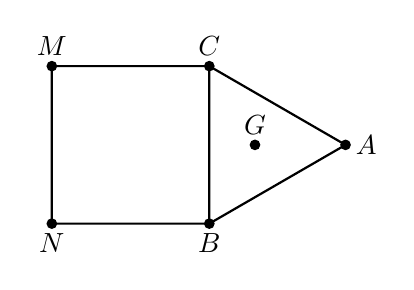
\begin{tikzpicture}[thick,,scale=1]
			\coordinate (A) at (4.73,-1); \coordinate (B) at (3,-2); \coordinate (C) at (3,0);
			\coordinate (M) at (1,0); \coordinate (N) at (1,-2); \coordinate (G) at (3.58,-1);
			\draw (A)--(B)--(C)--(A)--(C)--(M)--(N)--(B);
			\foreach \i in {B,N} \draw[fill] (\i) circle (1.5pt) node[below] {$\i$};
			\foreach \i in {C,G,M} \draw[fill]  (\i) circle (1.5pt) node[above] {$\i$};
			\foreach \i in {A} \draw[fill]  (\i) circle (1.5pt) node[right] {$\i$};
		\end{tikzpicture}
	}
	\loigiai{
		\begin{center}
			\begin{tikzpicture}[>=angle 45,x=1cm,y=1cm,scale=1.2]
				\coordinate (A) at (4.73,-1); \coordinate (B) at (3,-2); \coordinate (C) at (3,0);
				\coordinate (M) at (1,0); \coordinate (N) at (1,-2); \coordinate (G) at (3.58,-1);
				\coordinate (E) at (-1,-2); \coordinate (F) at (-1,-1);
				\draw[thick] (A)--(B)--(C)--(A)--(C)--(M)--(N)--(B) (E)--(F)--(G);
				\draw[->, thick] (C)--(M) ;\draw[->, thick] (N)--(E) ;
				\draw[->,thick] (G)--(N); \draw[->, thick] (G)--(E);
				\foreach \i in {B,N,E} \draw[fill] (\i) circle (1.5pt) node[below] {$\i$};
				\foreach \i in {C,G,M,F} \draw[fill]  (\i) circle (1.5pt) node[above] {$\i$};
				\foreach \i in {A} \draw[fill]  (\i) circle (1.5pt) node[right] {$\i$};
			\end{tikzpicture}
		\end{center}
		Ta có $\vec{GA} + \vec{GB} + \vec{GM} + \vec{GN} = \vec{CG} + \vec{GM} + \vec{GN} = \vec{CM} +\vec{GN}
		=\vec{NE} +\vec{GN} = \vec{GE}$ \\
		$|\vec{u}|=|\vec{GE}| = \sqrt{\dfrac{a^2}{4} + \left (2a+\dfrac{\sqrt{3}}{6}\right )^2}$
	}
\end{baitap} \cham{10}

\begin{baitap}
	\immini{Cho hai lực đồng quy $\overrightarrow{F_1}$ và $\overrightarrow{F_2}$ như hình vẽ. Biết độ lớn của $\overrightarrow{F_1},\text{ }\overrightarrow{F_2}$ lần lượt là 3N và 2N. Tính độ lớn hợp lực của $\overrightarrow{F_1}$ và $\overrightarrow{F_2}$.
	}{\hspace{1cm}
		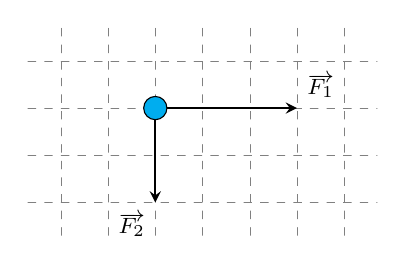
\begin{tikzpicture}[>=stealth,scale=0.6, line join=round, line cap=round]
			\draw[line width=0.05pt,gray,dashed] (-2.7,-0.7) grid (4.7,3.7);
			\draw[->,thick](0,2)--(0,0)node[below left]{\footnotesize$\overrightarrow{F_2}$};
			\draw[->,thick](0,2)--(3,2)node[above right]{\footnotesize$\overrightarrow{F_1}$};
			\draw[fill=cyan] (0,2) circle(7pt);
	\end{tikzpicture}}
\loigiai{
$\big|\vec{F_1}+\vec{F_2}\big|=\sqrt{3^2+2^2}=\sqrt{13}$ (N)
}
\end{baitap} \cham{2}

\begin{baitap}%[0H1K2-5]%
	\immini{Cho ba lực $\overrightarrow{F_1}=\overrightarrow{MA}$, $\overrightarrow{F_2}=\overrightarrow{MB}$, $\overrightarrow{F_3}=\overrightarrow{MC}$ cùng điểm đặt $M$, cùng tác động vào một vật và vật đó đứng yên (như hình vẽ). Biết cường độ của $\overrightarrow{F_1}$, $\overrightarrow{F_2}$ đều bằng $30$ N và $\widehat{AMB}=60^\circ$. Tính cường độ của lực $\overrightarrow{F_3}$.
	}{
\begin{tikzpicture}[smooth,font=\footnotesize,scale=0.8,>=Latex]
	\path
	(0,0) coordinate (M)
	(3,0) coordinate (M1)
	($(M)!1!30:(M1)$) coordinate (A)
	($(M)!1!-30:(M1)$) coordinate (B)
	($(A)+(B)-(M)$) coordinate (D)
	($(M)+(M)-(D)$) coordinate (C)
	;
	\fill[ball color=red](0,0) circle (0.16);
	\draw[->] (M)--(A);
	\draw[->] (M)--(B);
	\draw[->] (M)--(C);
	\foreach \x/\g in {A/90,B/-90,C/180,M/90} \draw [fill=black] (\x) circle (.05) + (\g:.5) node{$\x$};
	\begin{scope}
		\clip (B)--(M)--(A);
		\draw[double] (M) circle(0.6cm);
	\end{scope}
	\node[right] at (0.6,0) {$60^\circ$};
\end{tikzpicture}}
	\loigiai
	{
		\begin{center}
			\begin{tikzpicture}[smooth,font=\footnotesize,scale=0.8,>=Latex]
				\path
				(0,0) coordinate (M)
				(3,0) coordinate (M1)
				($(M)!1!30:(M1)$) coordinate (A)
				($(M)!1!-30:(M1)$) coordinate (B)
				($(A)+(B)-(M)$) coordinate (D)
				($(M)+(M)-(D)$) coordinate (C)
				;
				\fill[ball color=red](0,0) circle (0.16);
				\draw[->] (M)--(A);
				\draw[->] (M)--(B);
				\draw[->] (M)--(C);
				\draw[->] (M)--(D);
				\draw[dashed] (A)--(D)--(B);
				\foreach \x/\g in {A/90,B/-90,C/180,M/90,D/0} \draw [fill=black] (\x) circle (.05) + (\g:.5) node{$\x$};
				\begin{scope}
					\clip (B)--(M)--(A);
					\draw[double] (M) circle(0.6cm);
				\end{scope}
				\node[right] at (0.6,0) {$60^\circ$};
			\end{tikzpicture}
		\end{center}
		Dựng hình bình hành $ADBM$, lại có $MA=MB$ nên $ADBM$ là hình thoi. Suy ra $MD \perp AB$ và $MD=2MH$, với $H$ là giao điểm của $AB$ và $MD$.\\
		Tam giác $MAB$ có $MA=MB=30$ và $\widehat{AMB}=60^\circ$ nên $MAB$ là tam giác đều cạnh $30$.\\
		Khi đó $MH=\dfrac{30\sqrt{3}}{2}=15\sqrt{3}$ và $MD=30\sqrt{3}$.\\
		Ba lực $\overrightarrow{F_1}$, $\overrightarrow{F_2}$, $\overrightarrow{F_3}$ cùng tác động vào một vật và vật đó đứng yên khi và chỉ khi
		\allowdisplaybreaks
		\begin{eqnarray*}
			\overrightarrow{F_1}+\overrightarrow{F_2}+\overrightarrow{F_3}=\overrightarrow{0} \Leftrightarrow \overrightarrow{MA}+\overrightarrow{MB}+\overrightarrow{MC}=\overrightarrow{0} \Leftrightarrow \overrightarrow{MD}+\overrightarrow{MC}=\overrightarrow{0} \Leftrightarrow \overrightarrow{MC}=-\overrightarrow{MD}.
		\end{eqnarray*}
		Do đó cường độ lực $\overrightarrow{F_3}$ là $\left|\overrightarrow{MC}\right| = \left|-\overrightarrow{MD}\right|=\left|\overrightarrow{MD}\right| = MD = 30\sqrt{3}$ N.
	}
\end{baitap} \cham{13}

\begin{baitap}
	\immini{Trên hình bên biểu diễn ba lực $\vec{F_1}$, $\vec{F_2}$, $\vec{F_3}$ cùng tác động vào vật ở vị trí cân bằng $A$. Cho biết $\big|\vec{F_1}\big|=30N$, $\big|\vec{F_2}\big|=40N$. Tính cường độ của lực $\vec{F_3}$.
			}{\vspace{-1cm}\hspace{1cm}
				\begin{tikzpicture}[smooth,font=\footnotesize,scale=0.68,>=Latex]
				\path
				(0,0) coordinate (A)
				(1,1.5) coordinate (B)
				(4,-0.5) coordinate (C)
				(3,-2) coordinate (D)
				(-4,0.5) coordinate (E);
				\draw
				pic[draw, angle radius=2mm]{right angle=B--A--D};
				\draw[->] (A)--(B)node[shift={(-160:0.7)}]{\scriptsize$\vec{F_1}$};
				\draw[->] (A)--(D)node[shift={(200:0.6)}]{\scriptsize$\vec{F_2}$};
				\draw[->] (A)--(E)node[shift={(10:1)}]{\scriptsize$\vec{F_3}$};
				\foreach \x/\g in {A/-90,B/90,D/-90,E/-180} \draw [fill=black] (\x) circle (.05) + (\g:.4) node{$\x$};
			\end{tikzpicture}
			}
			\loigiai{
			Vật $A$ ở trạng thái cân bằng nên tổng các lực tác dụng lên vật bằng vectơ không. Ta có:
			$$ \overrightarrow{F_1} + \overrightarrow{F_2} + \overrightarrow{F_3} = \vec{0} \Leftrightarrow \overrightarrow{F_3} = -(\overrightarrow{F_1} + \overrightarrow{F_2}) $$
			Gọi $\overrightarrow{F_{12}} = \overrightarrow{F_1} + \overrightarrow{F_2}$ là hợp lực của hai lực $\overrightarrow{F_1}$ và $\overrightarrow{F_2}$.\\
			Khi đó, $\overrightarrow{F_3} = -\overrightarrow{F_{12}}$, tức là lực $\overrightarrow{F_3}$ trực đối với hợp lực $\overrightarrow{F_{12}}$.\\
			Suy ra cường độ của lực $\overrightarrow{F_3}$ bằng với cường độ của hợp lực $\overrightarrow{F_{12}}$:
			$$ |\overrightarrow{F_3}| = |\overrightarrow{F_{12}}| $$
			Mặt khác, theo giả thiết $\overrightarrow{F_1} \perp \overrightarrow{F_2}$ (quan sát kí hiệu góc vuông trên hình) nên hình bình hành tạo bởi hai vectơ lực này là một hình chữ nhật. Áp dụng định lý Pythagore, ta có:
			$$ |\overrightarrow{F_{12}}| = \sqrt{|\overrightarrow{F_1}|^2 + |\overrightarrow{F_2}|^2} = \sqrt{30^2 + 40^2} = \sqrt{900 + 1600} = \sqrt{2500} = 50\,(\mathrm{N}). $$
			Vậy cường độ của lực $\overrightarrow{F_3}$ là $50$.
		}
\end{baitap} \cham{16}